%%%%%%%%%%%%%% COPYRIGHT INFORMATION %%%%%%%%%%%%%%
% Template by
% Author: Sascha Frank 
% Nov. 2006
% University Freiburg 
% www.informatik.uni-freiburg.de/~frank/
% Distributed freely for non-commercial use

%%%%%%%%%%%%%%%%%%%%% PREAMBLE %%%%%%%%%%%%%%%%%%%%%
\documentclass{beamer}
\usepackage{beamerthemeshadow}
\usepackage{lmodern}
\usepackage{pifont}
\usepackage{color}

% include frame number on each frame
\setbeamertemplate{footline}{\quad \insertframenumber/\inserttotalframenumber}
\newcommand{\cmark}{\ding{51}} % check-mark
\newcommand{\xmark}{\ding{55}} % X-mark
\newcommand{\inv}{^{-1}}
\newcommand{\e}{\varepsilon}
\newcommand{\E}{\mathbb{E}}
\newcommand{\N}{\mathbb{N}}
\renewcommand{\P}{\mathbb{P}}
\newcommand{\R}{\mathbb{R}}
\newcommand{\Var}{\mathbb{V}}
\newcommand{\X}{\mathcal{X}}
\newcommand{\Y}{\mathcal{Y}}
\newcommand{\Z}{\mathcal{Z}}
\newcommand{\dist}{\operatorname{dist}}
\newcommand{\vi}{{\vec i}}

%%%%%%%%%%%%%%%%%%%%% DOCUMENT %%%%%%%%%%%%%%%%%%%%%
\begin{document}
\title{Exponential Concentration Inequality\\ for a R\'enyi-$\alpha$ Divergence
Estimator}
\author[Singh,P\'oczos]{Shashank Singh
\footnote{Carnegie Mellon University, Pittsburgh, PA, USA}
\and Barnab\'as P\'oczos $^1$}
\date{June 22, 2014}
\frame{\titlepage}

\section{Introduction}
\subsection{Problem}
\frame{\frametitle{Problem}
Given $\alpha \in [0,1) \cup (1,\infty)$, estimate the R\'enyi-$\alpha$
divergence
\[D_\alpha(p\|q)
    = \frac{1}{\alpha - 1} \log \int_\X
                    p^\alpha(x)q^{1 - \alpha}(x) \, dx,\]
between two unknown, continuous, nonparametric probability densities $p$ and
$q$ over $\X = [0,1]^d$, using $n$ samples from each density.
}

\subsection{Contribution}
\frame{\frametitle{Contribution}
\begin{itemize}
\item plug-in estimator of R\'enyi-$\alpha$ divergence based on kernel density
estimation
\item bound bias of the estimator
\item prove a concentration inequality
\item simple proof-of-concept experiment
\end{itemize}
}

\subsection{Motivation}
\frame{\frametitle{Motivation}
\begin{itemize}
\item `distributional' machine learning algorithms
\begin{itemize}
\item finite-dimensional feature vectors $\rightarrow$
distribution features
\end{itemize}
\pause
\item KL-divergence, entropy, and mutual information special cases
\begin{itemize}
\item applications to feature selection, clustering, ICA, etc.
\end{itemize}
\pause
\item with concentration inequality:
\begin{itemize}
\item can simultaneously bound error of multiple estimates (e.g., forest
density estimation)
\item can derive hypothesis test for independence
\end{itemize}
\end{itemize}
}

\subsection{Related Work}
\frame{\frametitle{Related Work}
\begin{itemize}
\item Few known rates
\item No estimators have concentration inequalities or other results describing
their distribution
%\item Optimal rates for estimating integral functionals of a \emph{single}
%density have been known for a while
%\begin{itemize}
%\item Only recently for divergences
%\end{itemize}
\end{itemize}
}

\section{Assumptions}
\subsection{Density Assumptions}
\frame{\frametitle{Smoothness (H\"older) Condition}
Same assumptions on $p$ and $q$.    \\
\vspace{10mm}
\pause
$\beta$-H\"older condition on $p$:
\begin{itemize}
\item $\beta,L > 0$,
$\ell := \lfloor \beta \rfloor$ (so $\beta - 1 \leq \ell < \beta$)
\end{itemize}
All $\ell$-order (mixed) partial derivatives of $p$ and $q$ exist and
\[\sup_{\substack{x \neq y \in \X\\|\vi| = \ell}}
    \frac{|D^\vi p(x) - D^\vi p(y)|}{\|x - y\|_r^{\beta - \ell}} \leq L.
\]
}

\frame{\frametitle{Boundedness}
There exist known $\kappa_1,\kappa_2 \in \R$ such that, $\forall x \in \X$,
\[0 < \kappa_1 \leq p(x),q(x) \leq \kappa_2 < +\infty.\]
\begin{itemize}
\item \emph{Existence} of $\kappa_2$ is trivial, but our estimator requires it
to be \emph{known} beforehand.
\item Assuming $\kappa_1$ for $q$ is natural (to ensure
$D_\alpha(p\|q) < +\infty$).
\item $\kappa_1$ for $p$ is technical, and can be weakened/eliminated in
certain cases.
\item Reason for working on finite measure domain $\X = [0,1]^d$.
\end{itemize}
}

\frame{\frametitle{Boundary Condition}
All derivatives of $p$ vanish at the boundary; i.e.,
\[\sup_{1 \leq |\vi| \leq \ell} |D^\vi p(x)| \to 0\]
as
\[\dist(x,\partial\X) \to 0.\]
\pause
Strong assumption, but needed to eliminate boundary bias.
}

\subsection{Kernel Assumptions}
\frame{\frametitle{Kernel Assumptions}
$K : \R \to \R$ with support in $[-1,1]$ and satisfies
\[\int_{-1}^1 K(u) \, du = 1
    \quad \mbox{ and } \quad
    \int_{-1}^1 u^jK(u) \, du = 0,
    \quad \forall j \in \{1,\cdots,\ell\}.
\]
}

\section{Estimator}
\subsection{Mirrored Kernel Density Estimate}
\frame{\frametitle{Mirrored Kernel Density Estimate}
\begin{figure}[h!]
  \centering
  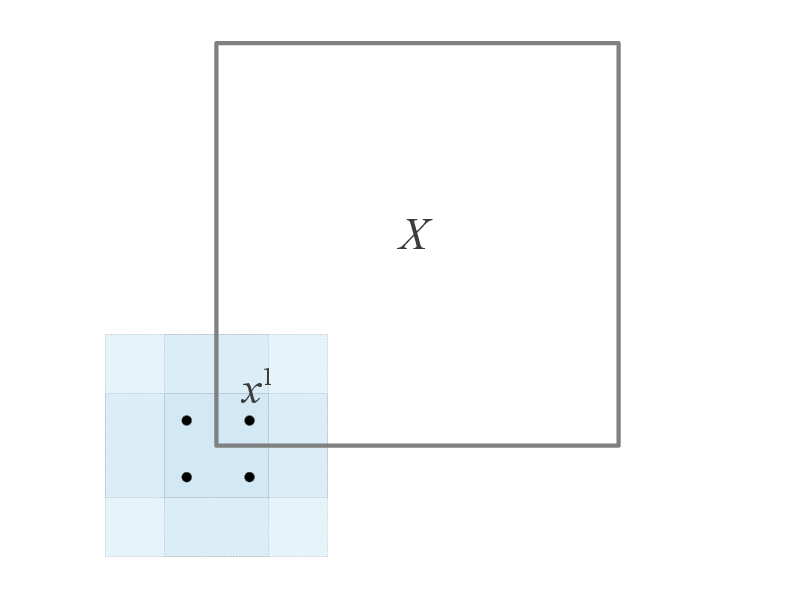
\includegraphics[width=0.6\linewidth]{mirror_fig}
%  \caption{\scriptsize Four kernels centered on a single data
%                       point and its three reflected copies,
%                       in the case $d = 2$.}
  \label{fig:mirror_fig}
\end{figure}
\vspace{-5mm}
\begin{enumerate}
\item Mirror data $x^1,\cdots,x^n$ across all subsets of edges of $\X$
\pause
\item Using a bandwidth $h$ and product kernel $K^d$, compute kernel density
estimate (KDE) $\widetilde{p}$ from resulting $3^dn$ data points
\pause
\begin{itemize}
\item Removes boundary bias because we assume derivatives of $p$ vanish near
$\partial\X$.
\end{itemize}
\end{enumerate}
}

\subsection{R\'enyi-$\alpha$ Divergence Estimator}
\frame{\frametitle{R\'enyi-$\alpha$ Divergence Estimator}
%TODO: set enum to 2 or 3, as appropraite
\begin{enumerate}
\item Clip mirrored KDE below by $\kappa_1$ and above by $\kappa_2$
\[\mbox{i.e.,} \quad
\hat p(x) = \min\{\kappa_2,\max\{\kappa_1,\widetilde{p}(x)\}\}.\]
\item Compute $\hat q$ by the same process
\item Plug $\hat p,\hat q$ into $D_\alpha$:
\[D_\alpha(\hat p\|\hat q)
    = \frac{1}{\alpha - 1} \log
        \int_\X \hat p^\alpha(x) \hat q^{1 - \alpha}(x) \, dx.
\]
\end{enumerate}
}

\section{Theoretical Results}
\frame{\frametitle{Bounds}
\begin{itemize}
\item {\bf Bias Bound:} $\exists C_B \in \R$ such that
\[|\E D_\alpha(\hat p\|\hat q) - D_\alpha(p\|q)|
\leq C_B\left( h^\beta + h^{2\beta} + \frac{1}{nh^d} \right).\]
\item {\bf Concentration Inequality (`Variance' Bound):}
$\exists C_V \in \R$ such that, $\forall \e > 0$,
\[\P\left(
        \left| D_\alpha(\hat p \| \hat q)
           - \E D_\alpha(\hat p \| \hat q) \right|
        > \e
    \right)
    \leq 2\exp\left( -C_V^2\e^2n \right).\]
\end{itemize}
}

\subsection{Bias Bound}
\frame{\frametitle{Bias Bound}
\[|\E D_\alpha(\hat p\|\hat q) - D_\alpha(p\|q)|
\leq C_B\left( h^\beta + h^{2\beta} + \frac{1}{nh^d} \right).\]
Proof Sketch:
\begin{enumerate}
\item Main step is to analyze boundary bias of mirrored KDE:
\[\int_\X (\E\hat p(x) - p(x))^2 \, dx \leq C_bh^{2\beta}.\]
\item Rest is a technical blend of standard proof techniques
\end{enumerate}
}

\subsection{Concentration Inequality}
\frame{\frametitle{Concentration Inequality}
  \[\P\left(
          \left| D_\alpha(\hat p \| \hat q)
             - \E D_\alpha(\hat p \| \hat q) \right|
          > \e
      \right)
      \leq 2\exp\left( -C_V^2\e^2n \right)\]
Proof Sketch:
\begin{itemize}
\pause
\item By McDiarmid's Inequality, suffices to bound change in estimator by
$C_V/n$ when resampling one data point.
\pause
\item By Mean Value Theorem, change is proportional to integrated change in
mirrored KDE.
\pause
\item By construction of KDE, this is proportional to $2\|K\|_1^d/n$.
\end{itemize}
}

\section{Consequences}
\frame{\frametitle{Consequences}
\begin{itemize}
\item Can bound variance by integrating concentration inequality:
\[\Var[D_\alpha(\hat p\|\hat q)] \leq C_V^2n\inv.\]
\pause
\item Choose bandwidth $h$ to minimize bias bound asymptotically:
$h \asymp n^{-\frac{1}{\beta + d}}$. Then,
\begin{itemize}
\item Bias is $O\left( n^{-\frac{\beta}{\beta + d}} \right)$
\item MSE is $O\left( n^{-\frac{2\beta}{\beta + d}} + n\inv\right)$
\item parametric rate $O(n\inv)$ if $\beta \geq d$ and slower
$O\left( n^{-\frac{2\beta}{\beta + d}} \right)$ else
\end{itemize}
\end{itemize}
}

\frame{\frametitle{Experiment Results}
Estimated divergence between two Gaussians in $\R^3$.
\begin{figure}[h!]
\centering
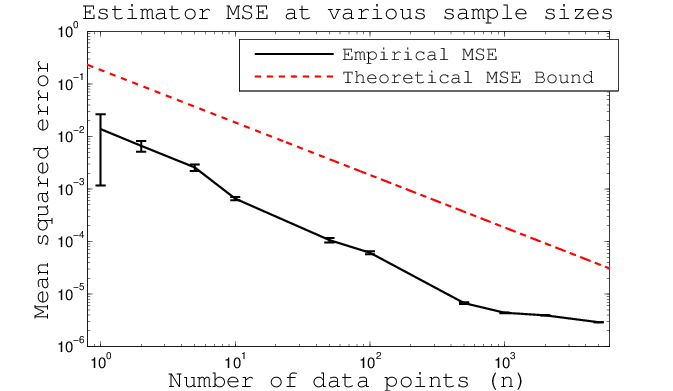
\includegraphics[width=0.8\linewidth]{MSE}
\caption{Log-log plot of empirical MSE alongside theoretical bound. Error
bars indicate standard deviation of estimator from 100 trials.}
\label{fig:exp_res}
\end{figure}
}

\frame{\frametitle{Summary}
\begin{itemize}
\item Present an estimator of R\'enyi-$\alpha$ Divergence
\pause
\item Prove $O\left( n^{-\frac{\beta}{\beta + d}} \right)$ bias bound
\pause
\item Prove exponential concentration of estimator
\pause
\item Experimentally verify results
\end{itemize}
}

\frame{\frametitle{Future Work}
\begin{enumerate}
%\item Improve rate to optimal $O\left( n^{-\frac{4\beta}{4\beta + d}} \right)$
%\begin{itemize}
%\item Try other approaches to bias bound
%\end{itemize}
\item Study role of dimension $d$
\item Prove concentration inequality for estimator of \emph{conditional}
quantities
\begin{itemize}
\item e.g., Conditional Mutual Information:
\[I_\alpha(X;Y|Z)
    = \int_\Z D_\alpha\left(P(X,Y|Z)\|P(X|Z)P(Y|Z)\right) \, dP(Z)
\]
\item hypothesis test for conditional independence
\end{itemize}
\end{enumerate}
}

\frame{\frametitle{\null}
\begin{center}
{\LARGE Thanks!}
\end{center}
}

\frame{\frametitle{References}
\begin{itemize}
\item $f$-Divergence estimation:
\begin{itemize}
\item Nguyen, X., Wainwright, M.J., and Jordan., M.I. Estimating divergence
functionals and the likelihood ratio by convex risk minimization. \emph{IEEE
Transactions on Information Theory}, 2010.
\end{itemize}
\item $k$-NN estimation:
\begin{itemize}
\item Poczos, B. and Schneider, J. On the estimation of alpha-divergences. In
\emph{International Conference on AI and Statistics (AISTATS)}, volume 15 of JMLR
Workshop and Conference Proceedings, pp. 609-617, 2011.
\end{itemize}
\item Lower bounds for single-density functional estimation:
\begin{itemize}
\item Birge, L. and Massart, P. Estimation of integral functions of a density.
\emph{The Annals of Statistics}, 23:11-29, 1995.
\end{itemize}
\item Distributional Machine Learning:
\begin{itemize}
\item Oliva, J., Poczos, B., and Schneider, J. Distribution to distribution
regression. In \emph{International Conference on Machine Learning (ICML)}, 2013.
\end{itemize}
\end{itemize}
}

\end{document}  
